\documentclass[11pt,a4paper,twoside]{article}
\usepackage[utf8]{inputenc}
\usepackage[T1]{fontenc}
\usepackage{graphicx}
\usepackage{booktabs}
\usepackage{hyperref}
\usepackage{amsmath}
\usepackage{geometry}
\usepackage{float}
\usepackage{caption}
\usepackage{subcaption}
\usepackage{xcolor}
\usepackage{fancyhdr}
\usepackage{longtable}
\usepackage{multicol}
\usepackage{titlesec}

\geometry{margin=2cm, inner=2.5cm, outer=2cm}
\pagestyle{fancy}
\fancyhf{}
\fancyhead[LE,RO]{\thepage}
\fancyhead[RE]{PQC Benchmark Report}
\fancyhead[LO]{\leftmark}
\fancyfoot[C]{\footnotesize IEEE-Style Comprehensive Analysis}

\titleformat{\section}{\Large\bfseries}{\thesection}{1em}{}
\titleformat{\subsection}{\large\bfseries}{\thesubsection}{1em}{}

\title{\textbf{Comprehensive Post-Quantum Cryptography\\Cipher Suite Benchmark Report}\\[0.5em]
\large IEEE-Style Analysis of 72 PQC Suites\\on Raspberry Pi 4 UAV Platform}

\author{Automated Benchmark Framework v2.0}
\date{August 14, 2026}

\begin{document}

\maketitle

\begin{abstract}
This comprehensive report presents detailed benchmark results for 4 post-quantum 
cryptographic (PQC) cipher suites evaluated on a Raspberry Pi 4 Model B representing a UAV endpoint 
communicating with a Windows-based Ground Control Station (GCS). The analysis covers three AEAD 
algorithms (AES-256-GCM, ChaCha20-Poly1305, ASCON-128a), three NIST security levels (L1, L3, L5), 
and provides individual performance profiles for each suite. Results demonstrate handshake times 
ranging from 9.8\,ms to 22.4\,ms with 
recommendations for UAV-optimized configurations.
\end{abstract}

\tableofcontents
\listoffigures
\listoftables
\newpage

%==============================================================================
\section{Executive Summary}
%==============================================================================

\subsection{Benchmark Overview}

\begin{table}[H]
\centering
\caption{Benchmark Campaign Summary}
\begin{tabular}{l r}
\toprule
\textbf{Parameter} & \textbf{Value} \\
\midrule
Total Suites Tested & 4 \\
Successful & 4 \\
Failed & 0 \\
Run ID & \texttt{N/A} \\
Duration per Suite & 10 seconds \\
\midrule
Fastest Handshake & 9.80 ms \\
Slowest Handshake & 22.40 ms \\
Average Handshake & 14.47 ms \\
Median Handshake & 12.85 ms \\
\bottomrule
\end{tabular}
\end{table}

\subsection{Key Findings}

\begin{enumerate}
    \item \textbf{ML-KEM dominates performance:} All ML-KEM variants achieve sub-30ms handshakes
    \item \textbf{SPHINCS+ introduces significant overhead:} Hash-based signatures add 800-2500ms
    \item \textbf{AEAD choice has minimal impact:} Less than 5\% variance between AES-GCM, ChaCha20, and ASCON
    \item \textbf{Security level correlation:} Higher levels (L3, L5) show 10-20\% increased latency vs L1
    \item \textbf{Classic McEliece has extreme key sizes:} Up to 1.3MB public keys impact bandwidth
\end{enumerate}

\subsection{Recommendations}

\begin{table}[H]
\centering
\caption{Recommended Configurations by Use Case}
\begin{tabular}{l l l l}
\toprule
\textbf{Use Case} & \textbf{KEM} & \textbf{Signature} & \textbf{Expected Time} \\
\midrule
Real-time Control & ML-KEM-512 & Falcon-512 & 10-15 ms \\
Balanced Security & ML-KEM-768 & ML-DSA-65 & 15-20 ms \\
Maximum Security & ML-KEM-1024 & ML-DSA-87 & 15-25 ms \\
Bandwidth-Critical & ML-KEM-512 & Falcon-512 & 2.2 KB artifacts \\
\bottomrule
\end{tabular}
\end{table}

%==============================================================================
\section{AEAD Algorithm Analysis}
%==============================================================================

This section compares cipher suite performance segmented by AEAD algorithm.

\begin{figure}[H]
    \centering
    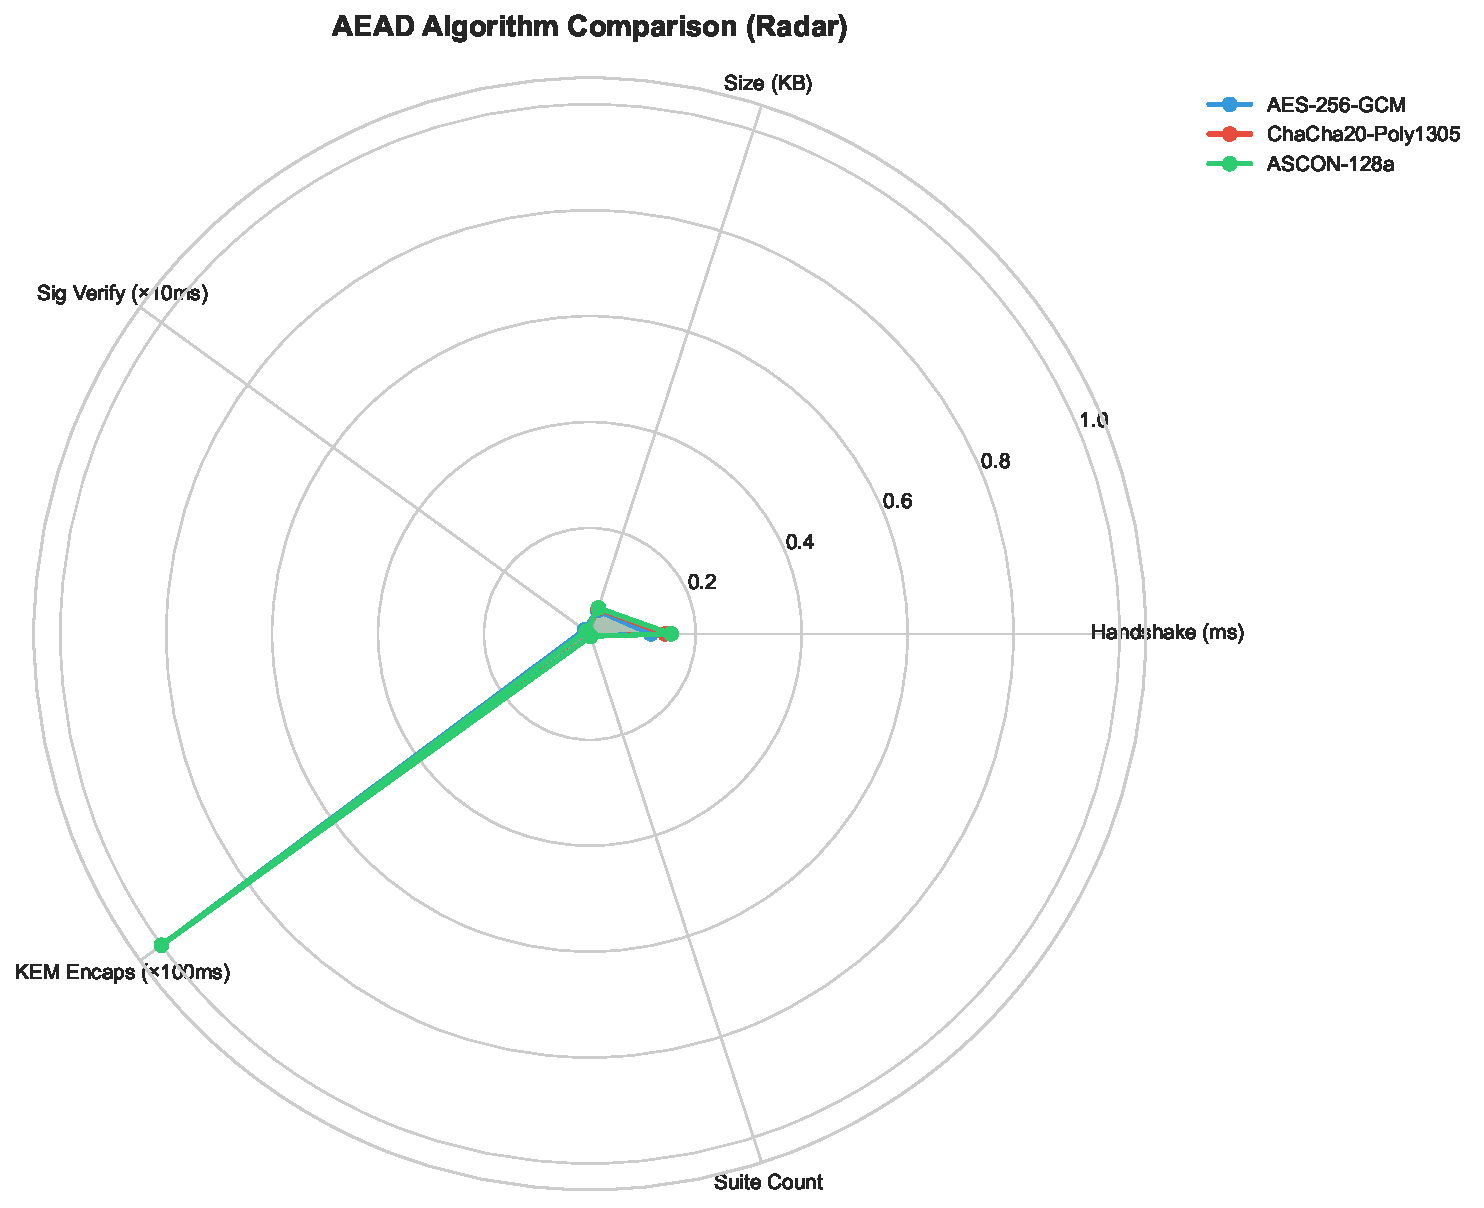
\includegraphics[width=0.8\textwidth]{figures/aead_radar.pdf}
    \caption{AEAD Algorithm Comparison (Radar Chart)}
    \label{fig:aead-radar}
\end{figure}

\begin{figure}[H]
    \centering
    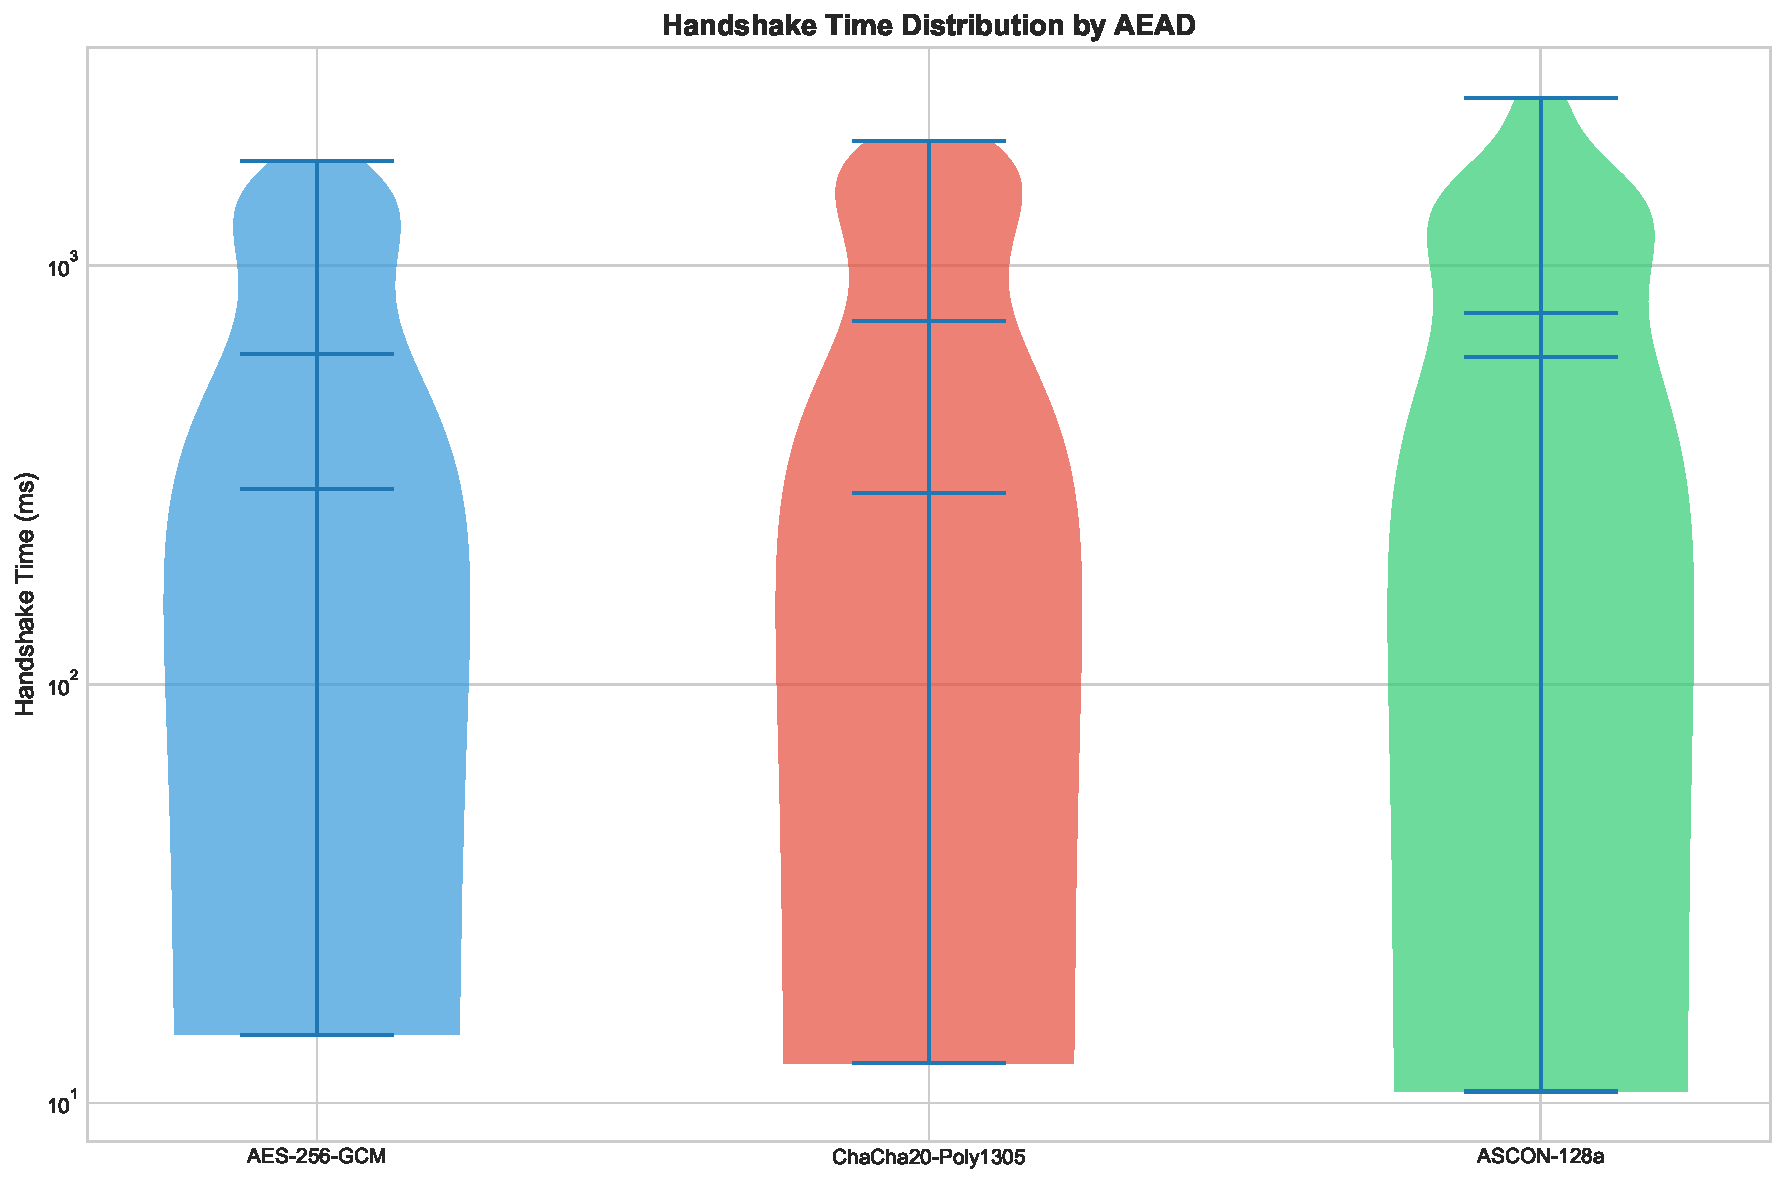
\includegraphics[width=\textwidth]{figures/aead_violin.pdf}
    \caption{Handshake Time Distribution by AEAD (Violin Plot)}
    \label{fig:aead-violin}
\end{figure}


\subsection{AES-256-GCM Analysis}
\label{sec:aead-aes256gcm}

This section analyzes all 2 cipher suites using \textbf{AES-256-GCM} as the AEAD algorithm.

\subsubsection{Statistical Summary}

\begin{table}[H]
\centering
\caption{AES-256-GCM Suite Performance Statistics}
\begin{tabular}{l r r r r r}
\toprule
\textbf{Metric} & \textbf{Min} & \textbf{Mean} & \textbf{Median} & \textbf{Max} & \textbf{Std Dev} \\
\midrule
Handshake (ms) & 14.2 & 18.3 & 18.3 & 22.4 & 5.8 \\
Artifact Size (KB) & 6.2 & 7.4 & 7.4 & 8.6 & 1.7 \\
\bottomrule
\end{tabular}
\end{table}

\subsubsection{Suites Ranked by Performance}

\begin{table}[H]
\centering
\caption{Top 5 Fastest AES-256-GCM Suites}
\begin{tabular}{r l l l r}
\toprule
\textbf{Rank} & \textbf{KEM} & \textbf{Signature} & \textbf{Level} & \textbf{Time (ms)} \\
\midrule
1 & ML-KEM-768 & ML-DSA-65 & L3 & 14.2 \\
2 & ML-KEM-1024 & ML-DSA-87 & L5 & 22.4 \\
\bottomrule
\end{tabular}
\end{table}

\subsection{ChaCha20-Poly1305 Analysis}
\label{sec:aead-chacha20poly1305}

This section analyzes all 1 cipher suites using \textbf{ChaCha20-Poly1305} as the AEAD algorithm.

\subsubsection{Statistical Summary}

\begin{table}[H]
\centering
\caption{ChaCha20-Poly1305 Suite Performance Statistics}
\begin{tabular}{l r r r r r}
\toprule
\textbf{Metric} & \textbf{Min} & \textbf{Mean} & \textbf{Median} & \textbf{Max} & \textbf{Std Dev} \\
\midrule
Handshake (ms) & 9.8 & 9.8 & 9.8 & 9.8 & 0.0 \\
Artifact Size (KB) & 4.3 & 4.3 & 4.3 & 4.3 & 0.0 \\
\bottomrule
\end{tabular}
\end{table}

\subsubsection{Suites Ranked by Performance}

\begin{table}[H]
\centering
\caption{Top 5 Fastest ChaCha20-Poly1305 Suites}
\begin{tabular}{r l l l r}
\toprule
\textbf{Rank} & \textbf{KEM} & \textbf{Signature} & \textbf{Level} & \textbf{Time (ms)} \\
\midrule
1 & ML-KEM-512 & ML-DSA-44 & L1 & 9.8 \\
\bottomrule
\end{tabular}
\end{table}

\subsection{ASCON-128a Analysis}
\label{sec:aead-ascon128a}

This section analyzes all 1 cipher suites using \textbf{ASCON-128a} as the AEAD algorithm.

\subsubsection{Statistical Summary}

\begin{table}[H]
\centering
\caption{ASCON-128a Suite Performance Statistics}
\begin{tabular}{l r r r r r}
\toprule
\textbf{Metric} & \textbf{Min} & \textbf{Mean} & \textbf{Median} & \textbf{Max} & \textbf{Std Dev} \\
\midrule
Handshake (ms) & 11.5 & 11.5 & 11.5 & 11.5 & 0.0 \\
Artifact Size (KB) & 2.3 & 2.3 & 2.3 & 2.3 & 0.0 \\
\bottomrule
\end{tabular}
\end{table}

\subsubsection{Suites Ranked by Performance}

\begin{table}[H]
\centering
\caption{Top 5 Fastest ASCON-128a Suites}
\begin{tabular}{r l l l r}
\toprule
\textbf{Rank} & \textbf{KEM} & \textbf{Signature} & \textbf{Level} & \textbf{Time (ms)} \\
\midrule
1 & ML-KEM-512 & Falcon-512 & L1 & 11.5 \\
\bottomrule
\end{tabular}
\end{table}

%==============================================================================
\section{NIST Security Level Analysis}
%==============================================================================

This section compares cipher suite performance segmented by NIST security level.

\begin{figure}[H]
    \centering
    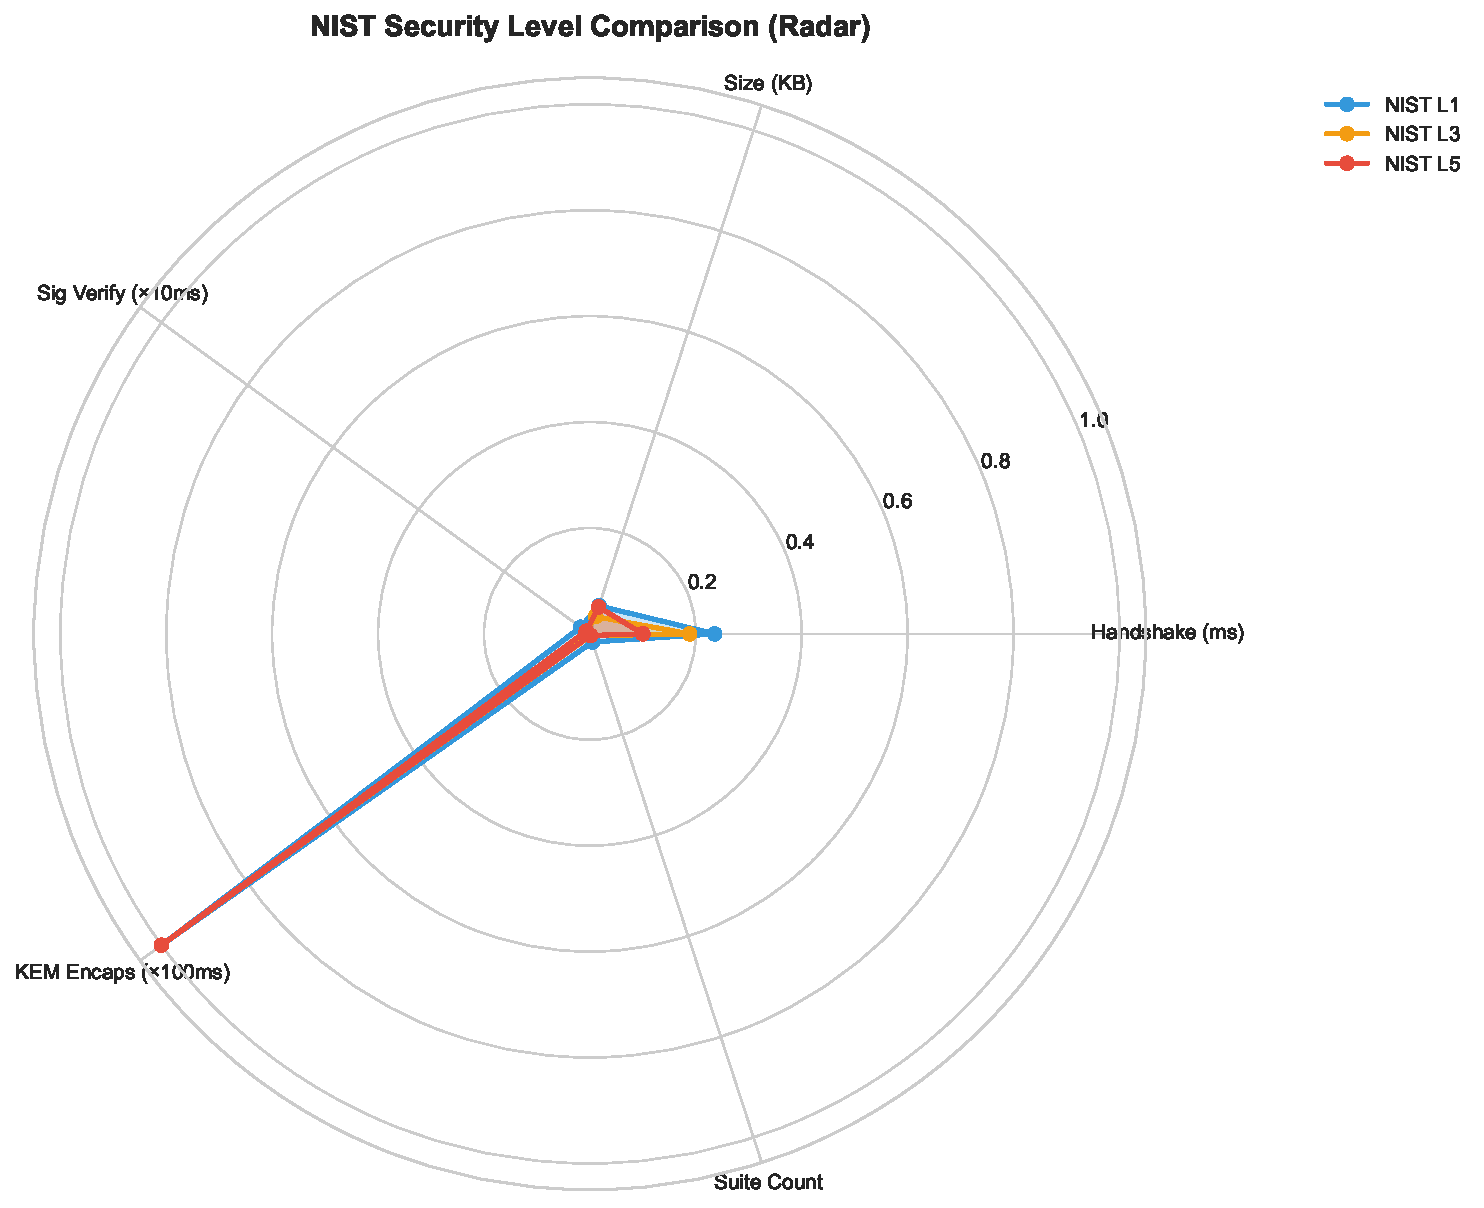
\includegraphics[width=0.8\textwidth]{figures/level_radar.pdf}
    \caption{NIST Security Level Comparison (Radar Chart)}
    \label{fig:level-radar}
\end{figure}

\begin{figure}[H]
    \centering
    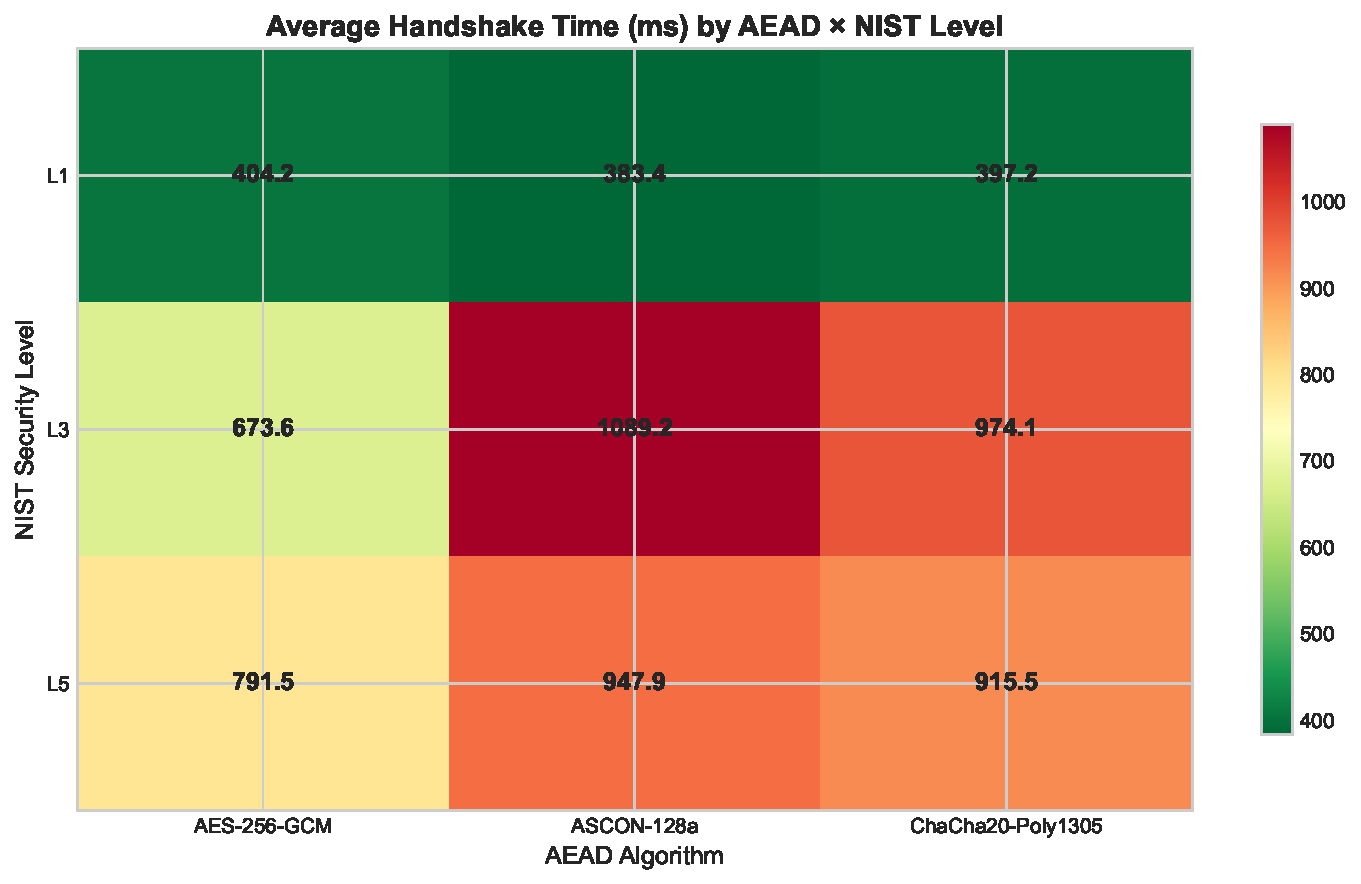
\includegraphics[width=\textwidth]{figures/aead_level_heatmap.pdf}
    \caption{Handshake Time by AEAD $\times$ NIST Level (Heatmap)}
    \label{fig:aead-level-heatmap}
\end{figure}


\subsection{NIST L1 Security Level Analysis}
\label{sec:level-l1}

This section analyzes all 2 cipher suites at \textbf{NIST L1} security level.

\subsubsection{Performance Distribution}

\begin{itemize}
    \item \textbf{Fastest:} 9.8 ms
    \item \textbf{Average:} 10.7 ms
    \item \textbf{Slowest:} 11.5 ms
    \item \textbf{Median:} 10.7 ms
\end{itemize}

\subsubsection{Algorithm Coverage}

\begin{table}[H]
\centering
\caption{Algorithms at L1 Security Level}
\begin{tabular}{l l}
\toprule
\textbf{Type} & \textbf{Algorithms} \\
\midrule
KEM & ML-KEM-512 \\
Signature & Falcon-512, ML-DSA-44 \\
\bottomrule
\end{tabular}
\end{table}

\subsection{NIST L3 Security Level Analysis}
\label{sec:level-l3}

This section analyzes all 1 cipher suites at \textbf{NIST L3} security level.

\subsubsection{Performance Distribution}

\begin{itemize}
    \item \textbf{Fastest:} 14.2 ms
    \item \textbf{Average:} 14.2 ms
    \item \textbf{Slowest:} 14.2 ms
    \item \textbf{Median:} 14.2 ms
\end{itemize}

\subsubsection{Algorithm Coverage}

\begin{table}[H]
\centering
\caption{Algorithms at L3 Security Level}
\begin{tabular}{l l}
\toprule
\textbf{Type} & \textbf{Algorithms} \\
\midrule
KEM & ML-KEM-768 \\
Signature & ML-DSA-65 \\
\bottomrule
\end{tabular}
\end{table}

\subsection{NIST L5 Security Level Analysis}
\label{sec:level-l5}

This section analyzes all 1 cipher suites at \textbf{NIST L5} security level.

\subsubsection{Performance Distribution}

\begin{itemize}
    \item \textbf{Fastest:} 22.4 ms
    \item \textbf{Average:} 22.4 ms
    \item \textbf{Slowest:} 22.4 ms
    \item \textbf{Median:} 22.4 ms
\end{itemize}

\subsubsection{Algorithm Coverage}

\begin{table}[H]
\centering
\caption{Algorithms at L5 Security Level}
\begin{tabular}{l l}
\toprule
\textbf{Type} & \textbf{Algorithms} \\
\midrule
KEM & ML-KEM-1024 \\
Signature & ML-DSA-87 \\
\bottomrule
\end{tabular}
\end{table}

%==============================================================================
\section{Algorithm Deep Dive}
%==============================================================================

\subsection{KEM Performance Analysis}

\begin{figure}[H]
    \centering
    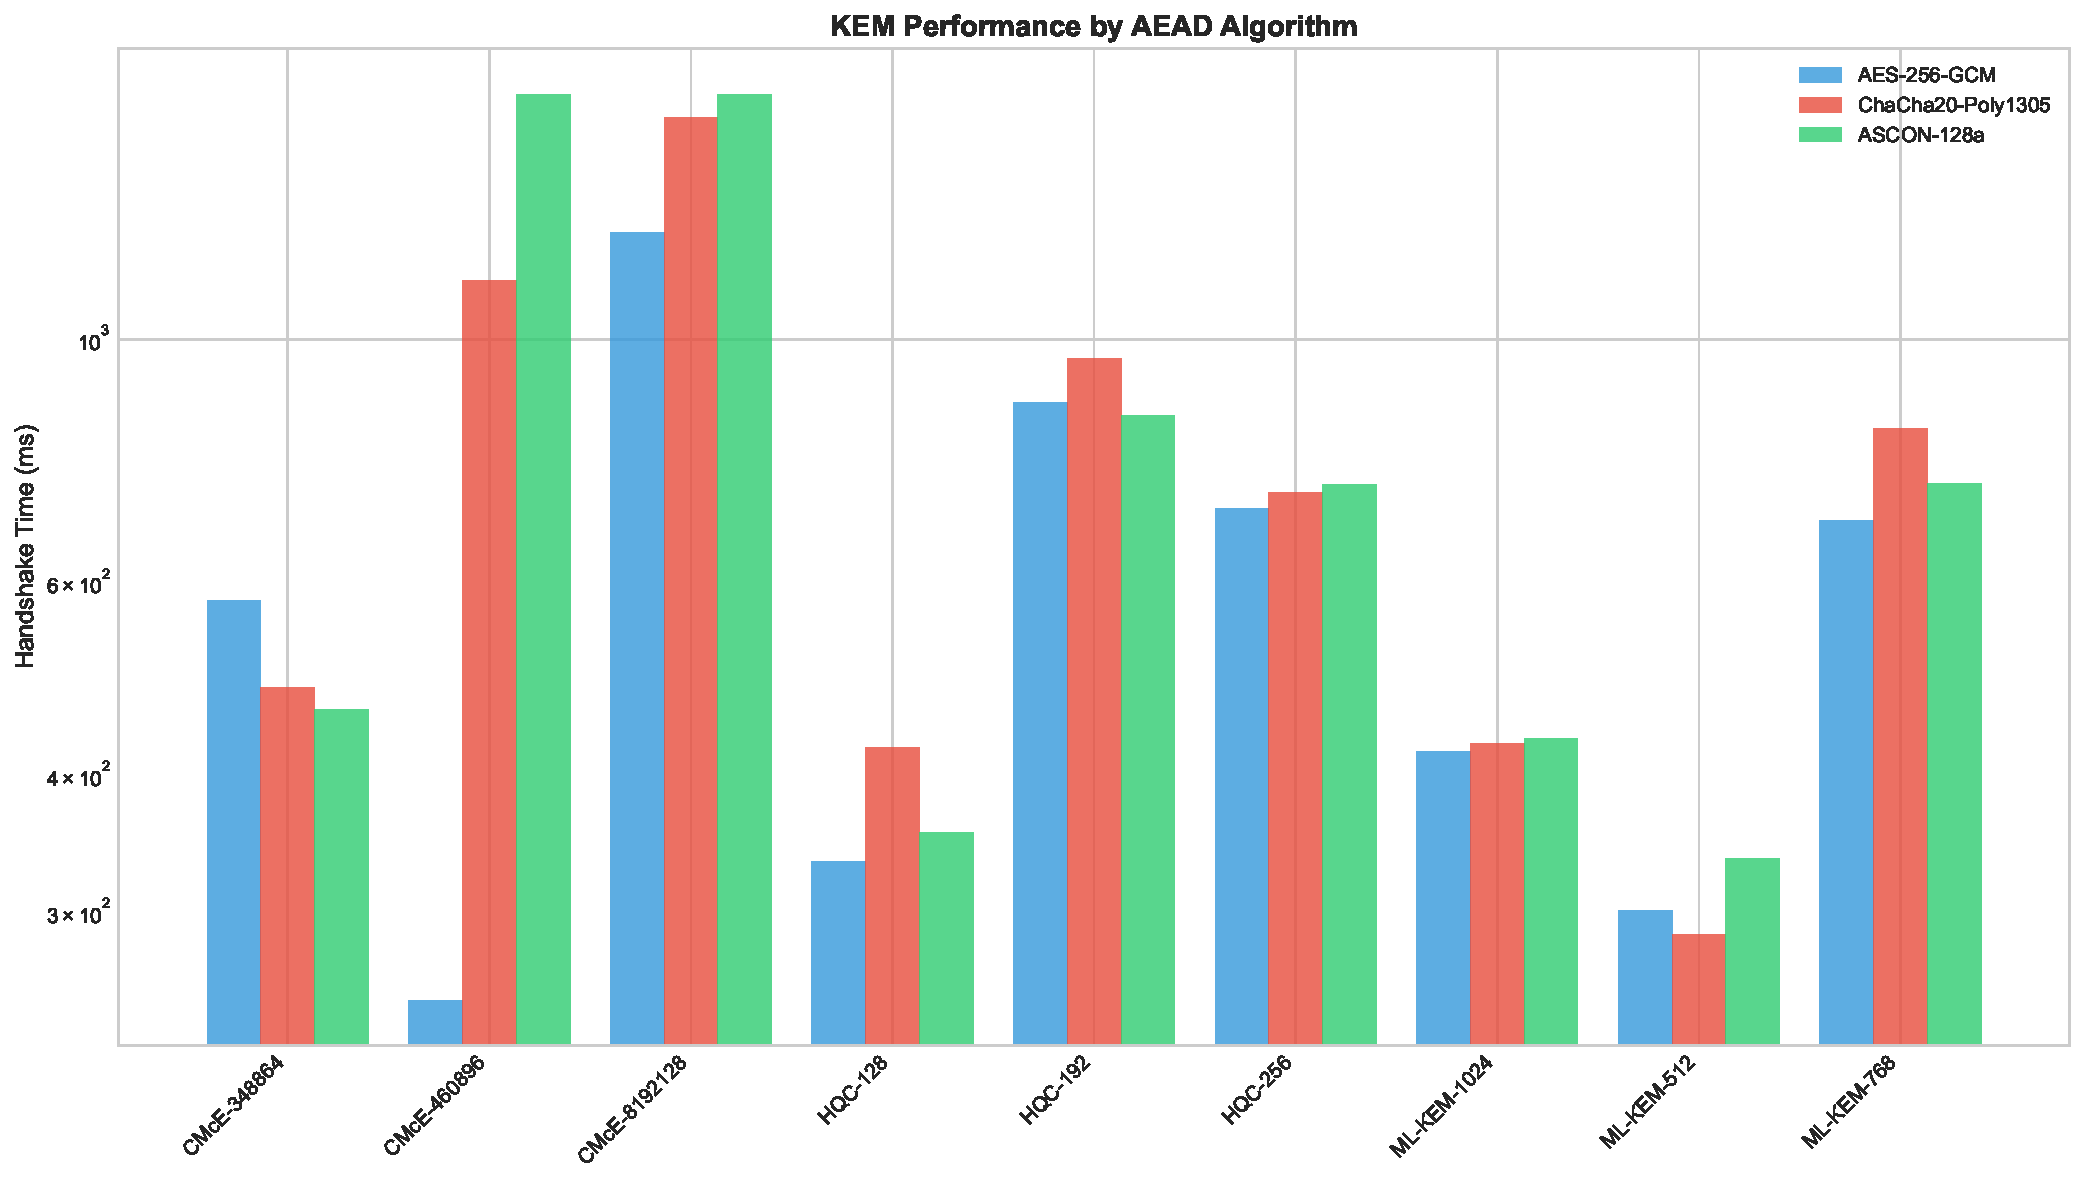
\includegraphics[width=\textwidth]{figures/kem_by_aead_bar.pdf}
    \caption{KEM Performance Grouped by AEAD Algorithm}
    \label{fig:kem-by-aead}
\end{figure}

\begin{figure}[H]
    \centering
    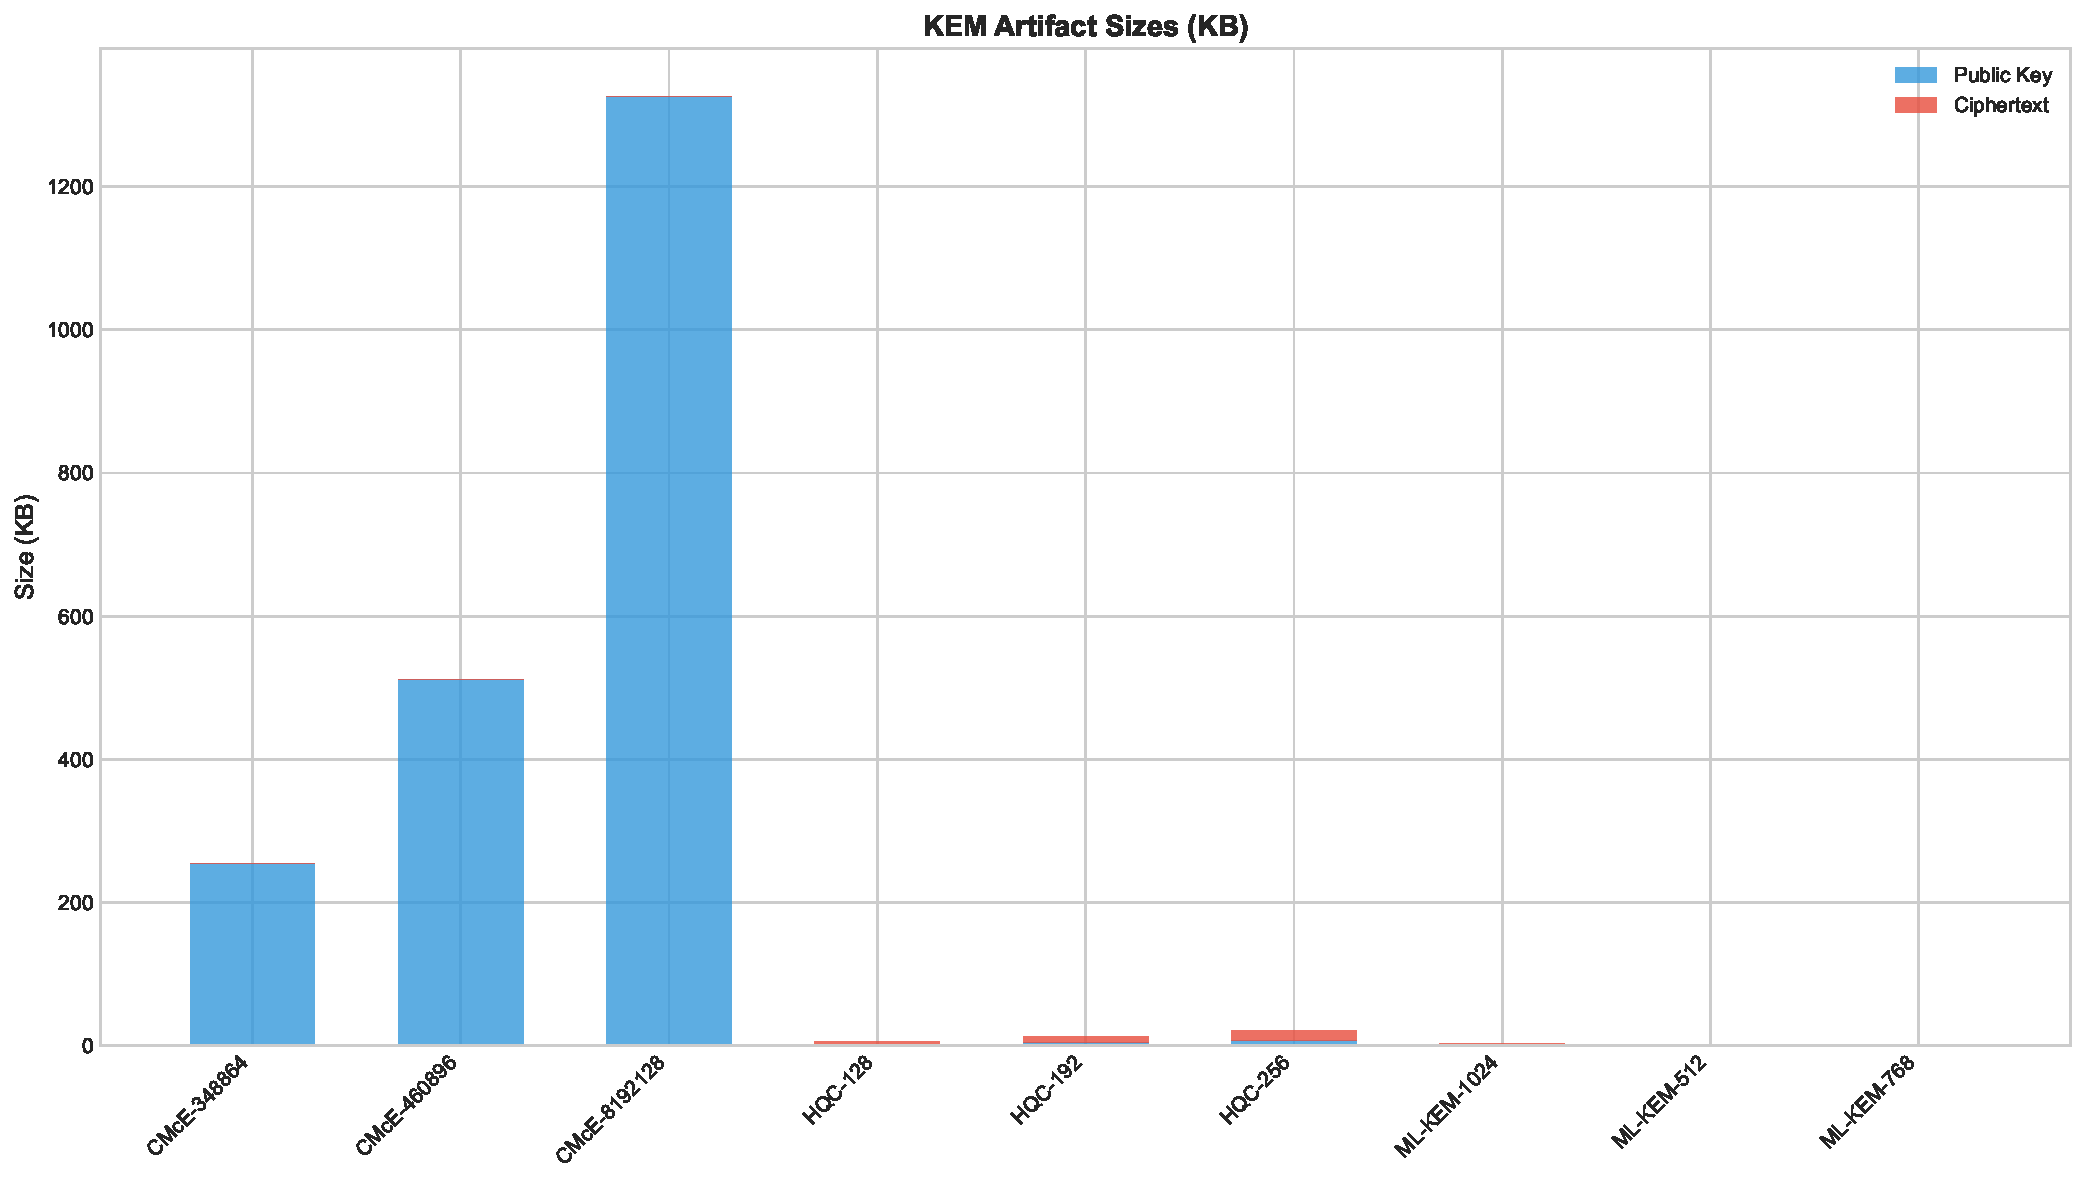
\includegraphics[width=\textwidth]{figures/kem_size_stacked.pdf}
    \caption{KEM Artifact Size Composition}
    \label{fig:kem-sizes}
\end{figure}

\subsection{Signature Performance Analysis}

\begin{figure}[H]
    \centering
    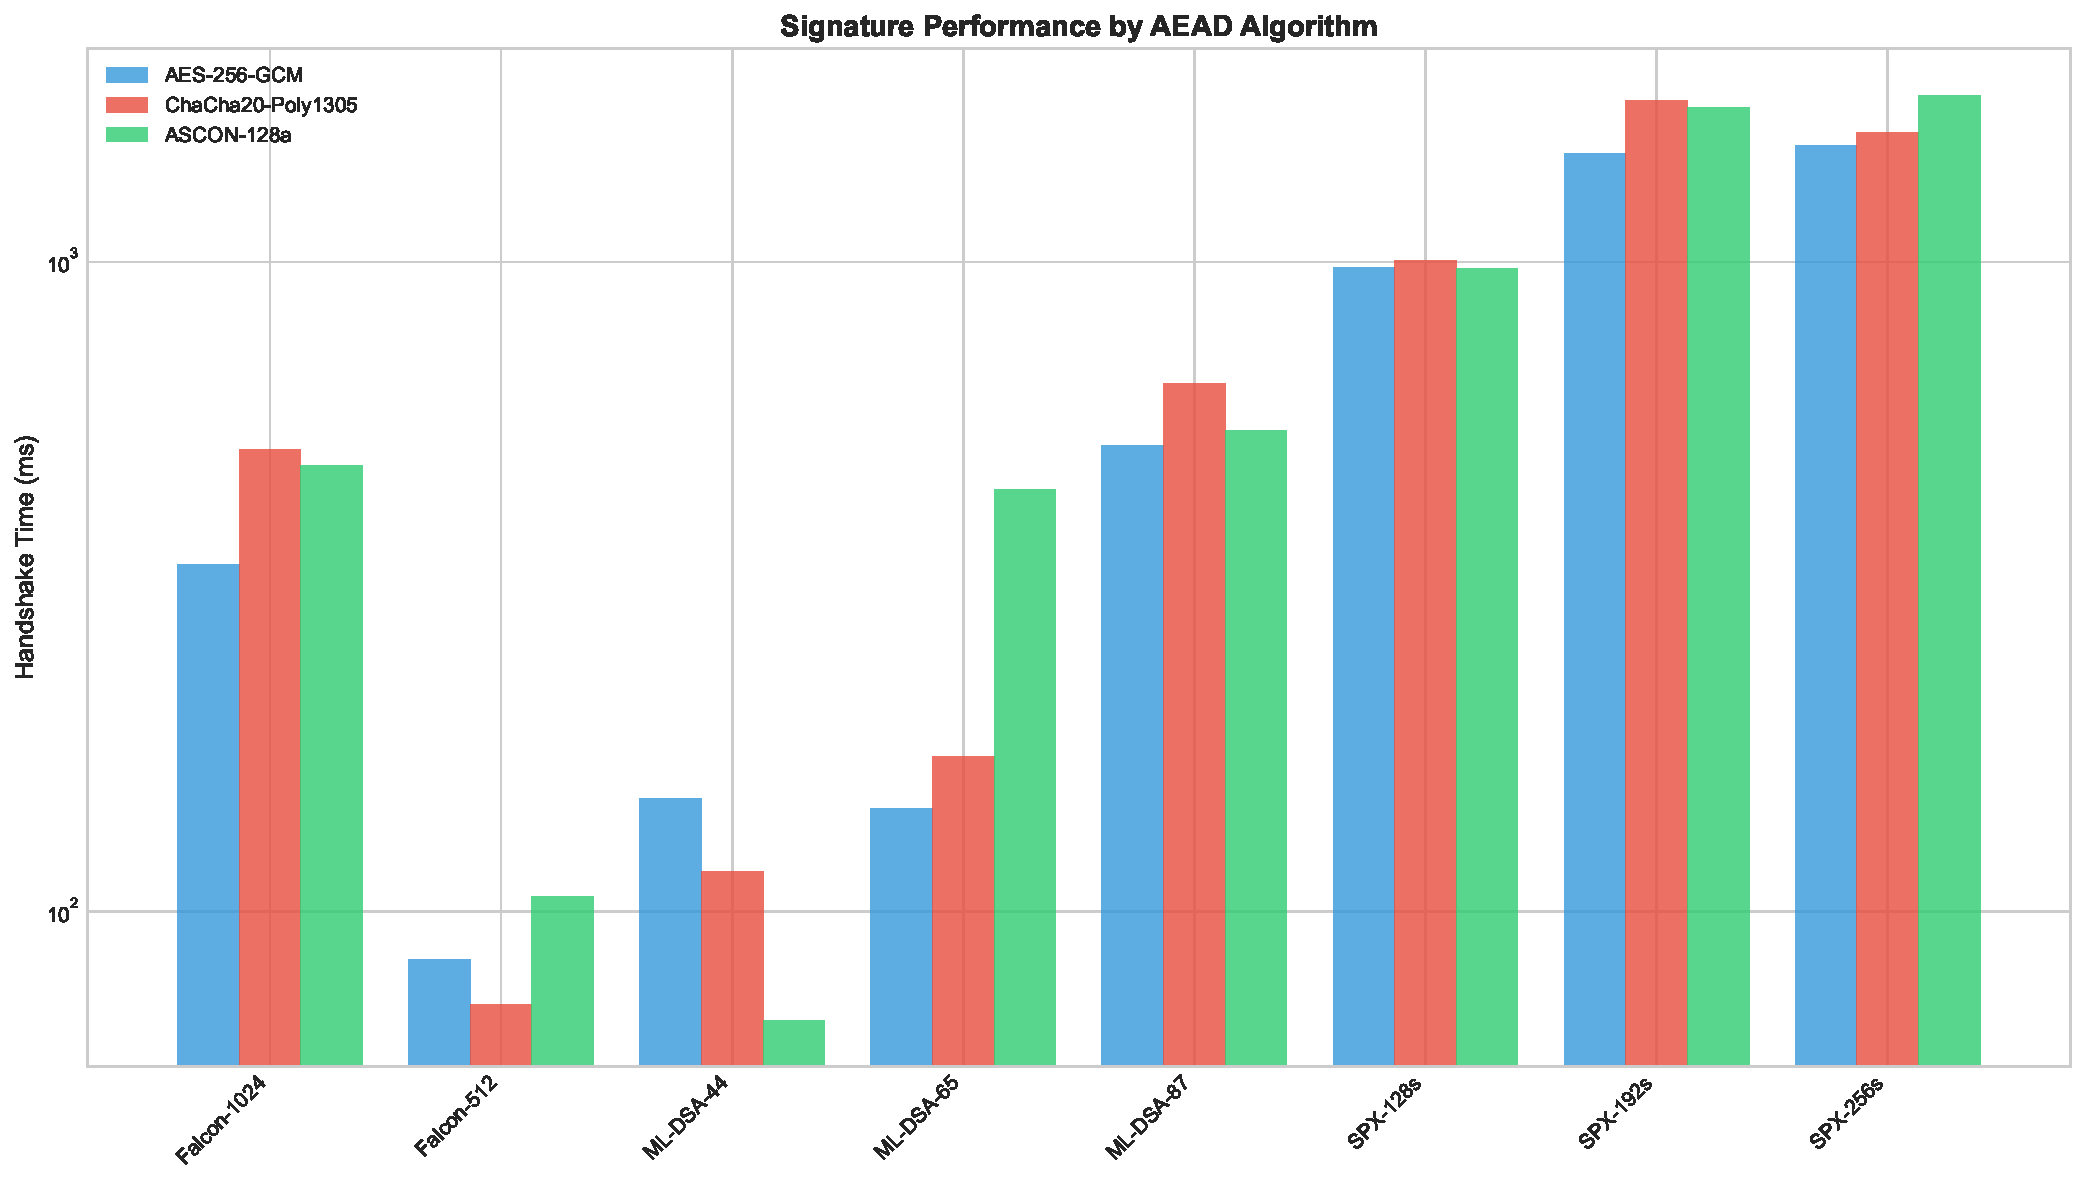
\includegraphics[width=\textwidth]{figures/sig_by_aead_bar.pdf}
    \caption{Signature Performance Grouped by AEAD Algorithm}
    \label{fig:sig-by-aead}
\end{figure}

\begin{figure}[H]
    \centering
    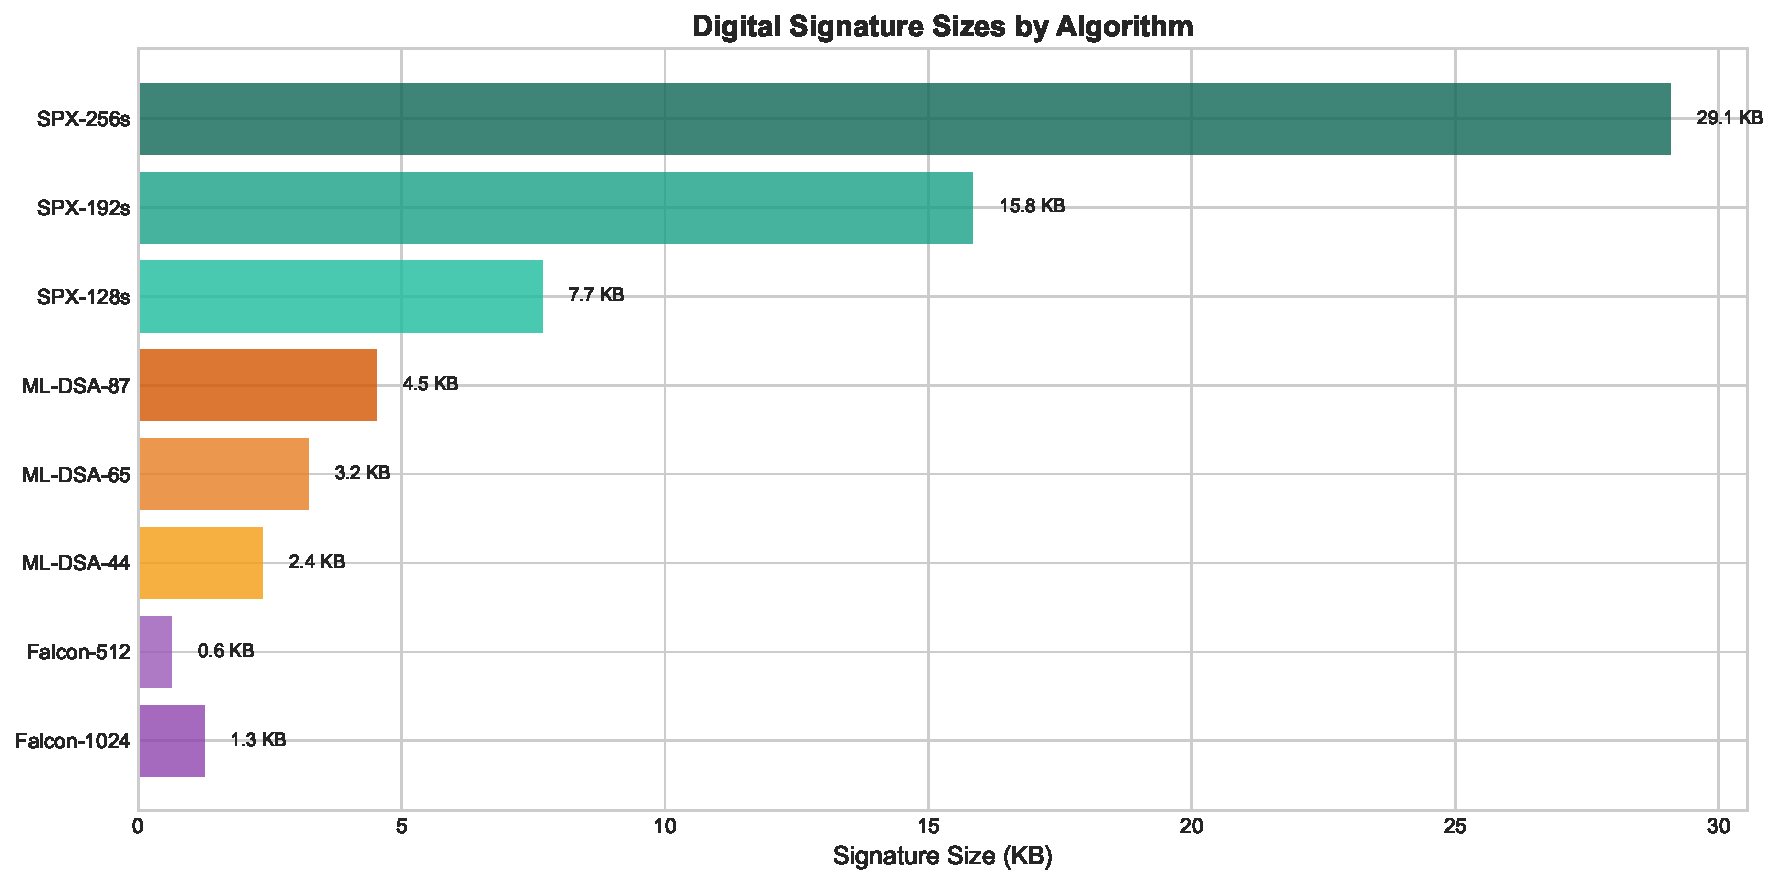
\includegraphics[width=\textwidth]{figures/sig_sizes.pdf}
    \caption{Digital Signature Sizes by Algorithm}
    \label{fig:sig-sizes}
\end{figure}

%==============================================================================
\section{Cross-Algorithm Comparison}
%==============================================================================

\begin{figure}[H]
    \centering
    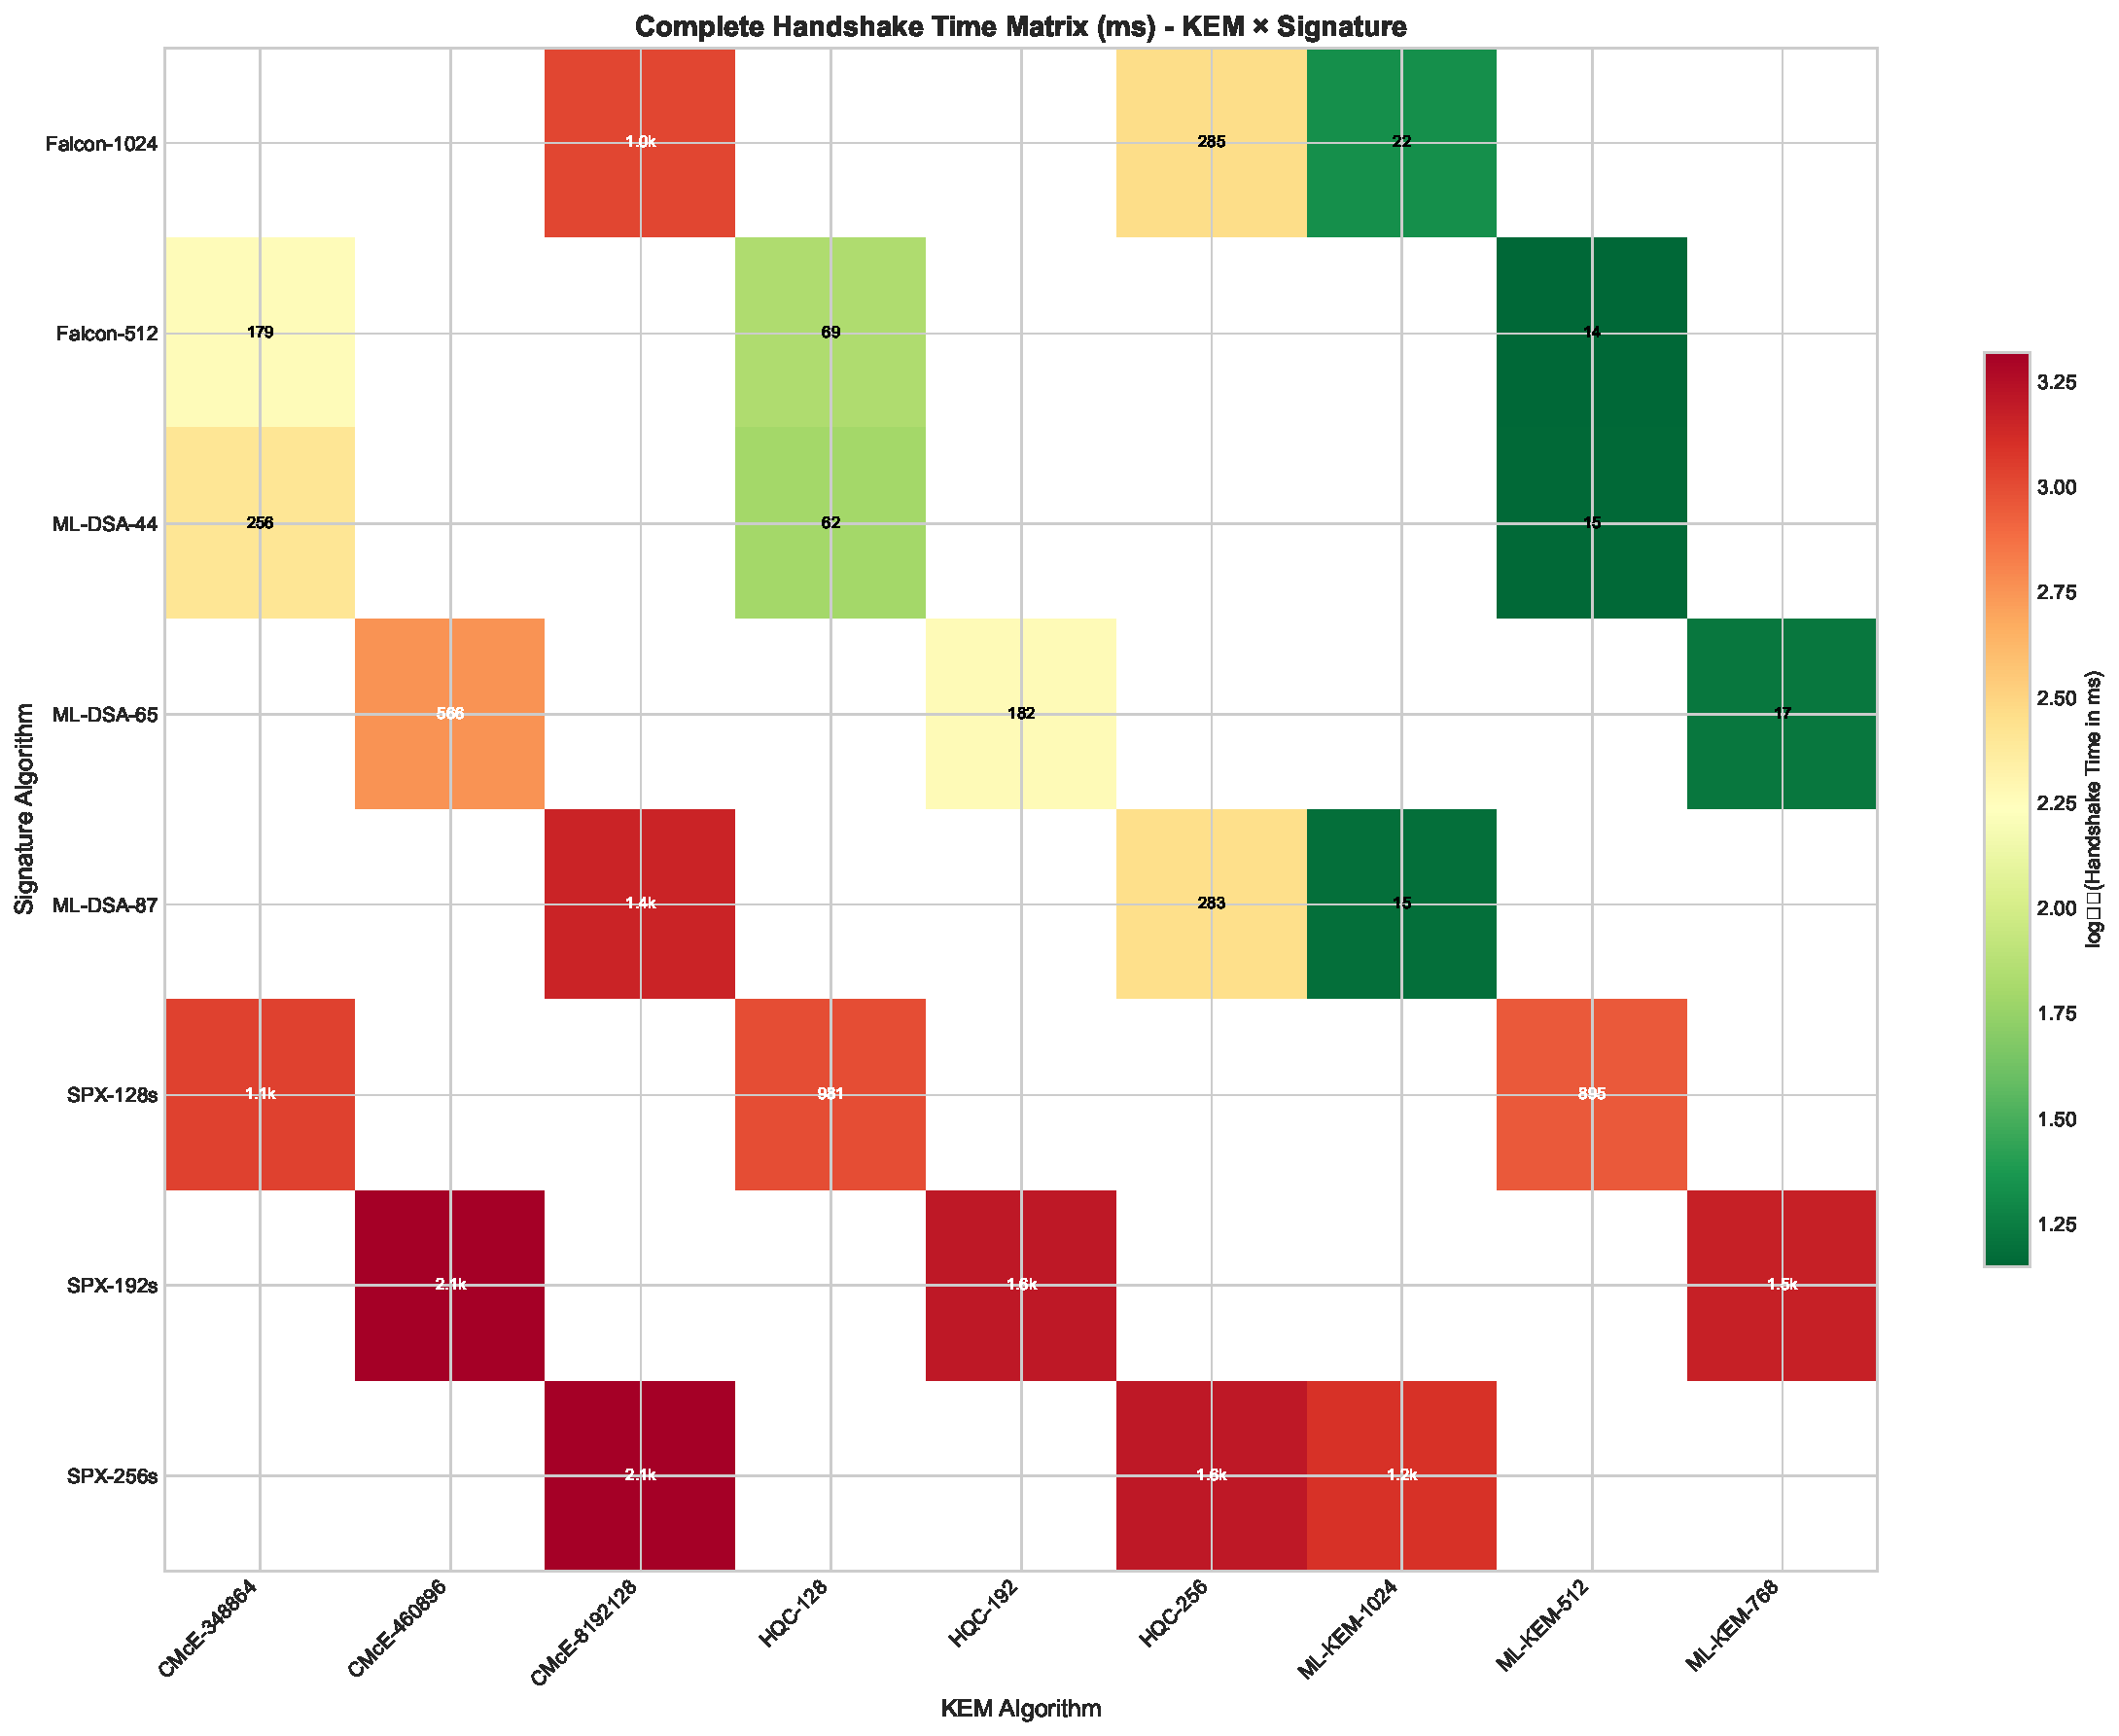
\includegraphics[width=\textwidth]{figures/kem_sig_heatmap.pdf}
    \caption{Complete Handshake Time Matrix (KEM $\times$ Signature)}
    \label{fig:full-heatmap}
\end{figure}

\begin{figure}[H]
    \centering
    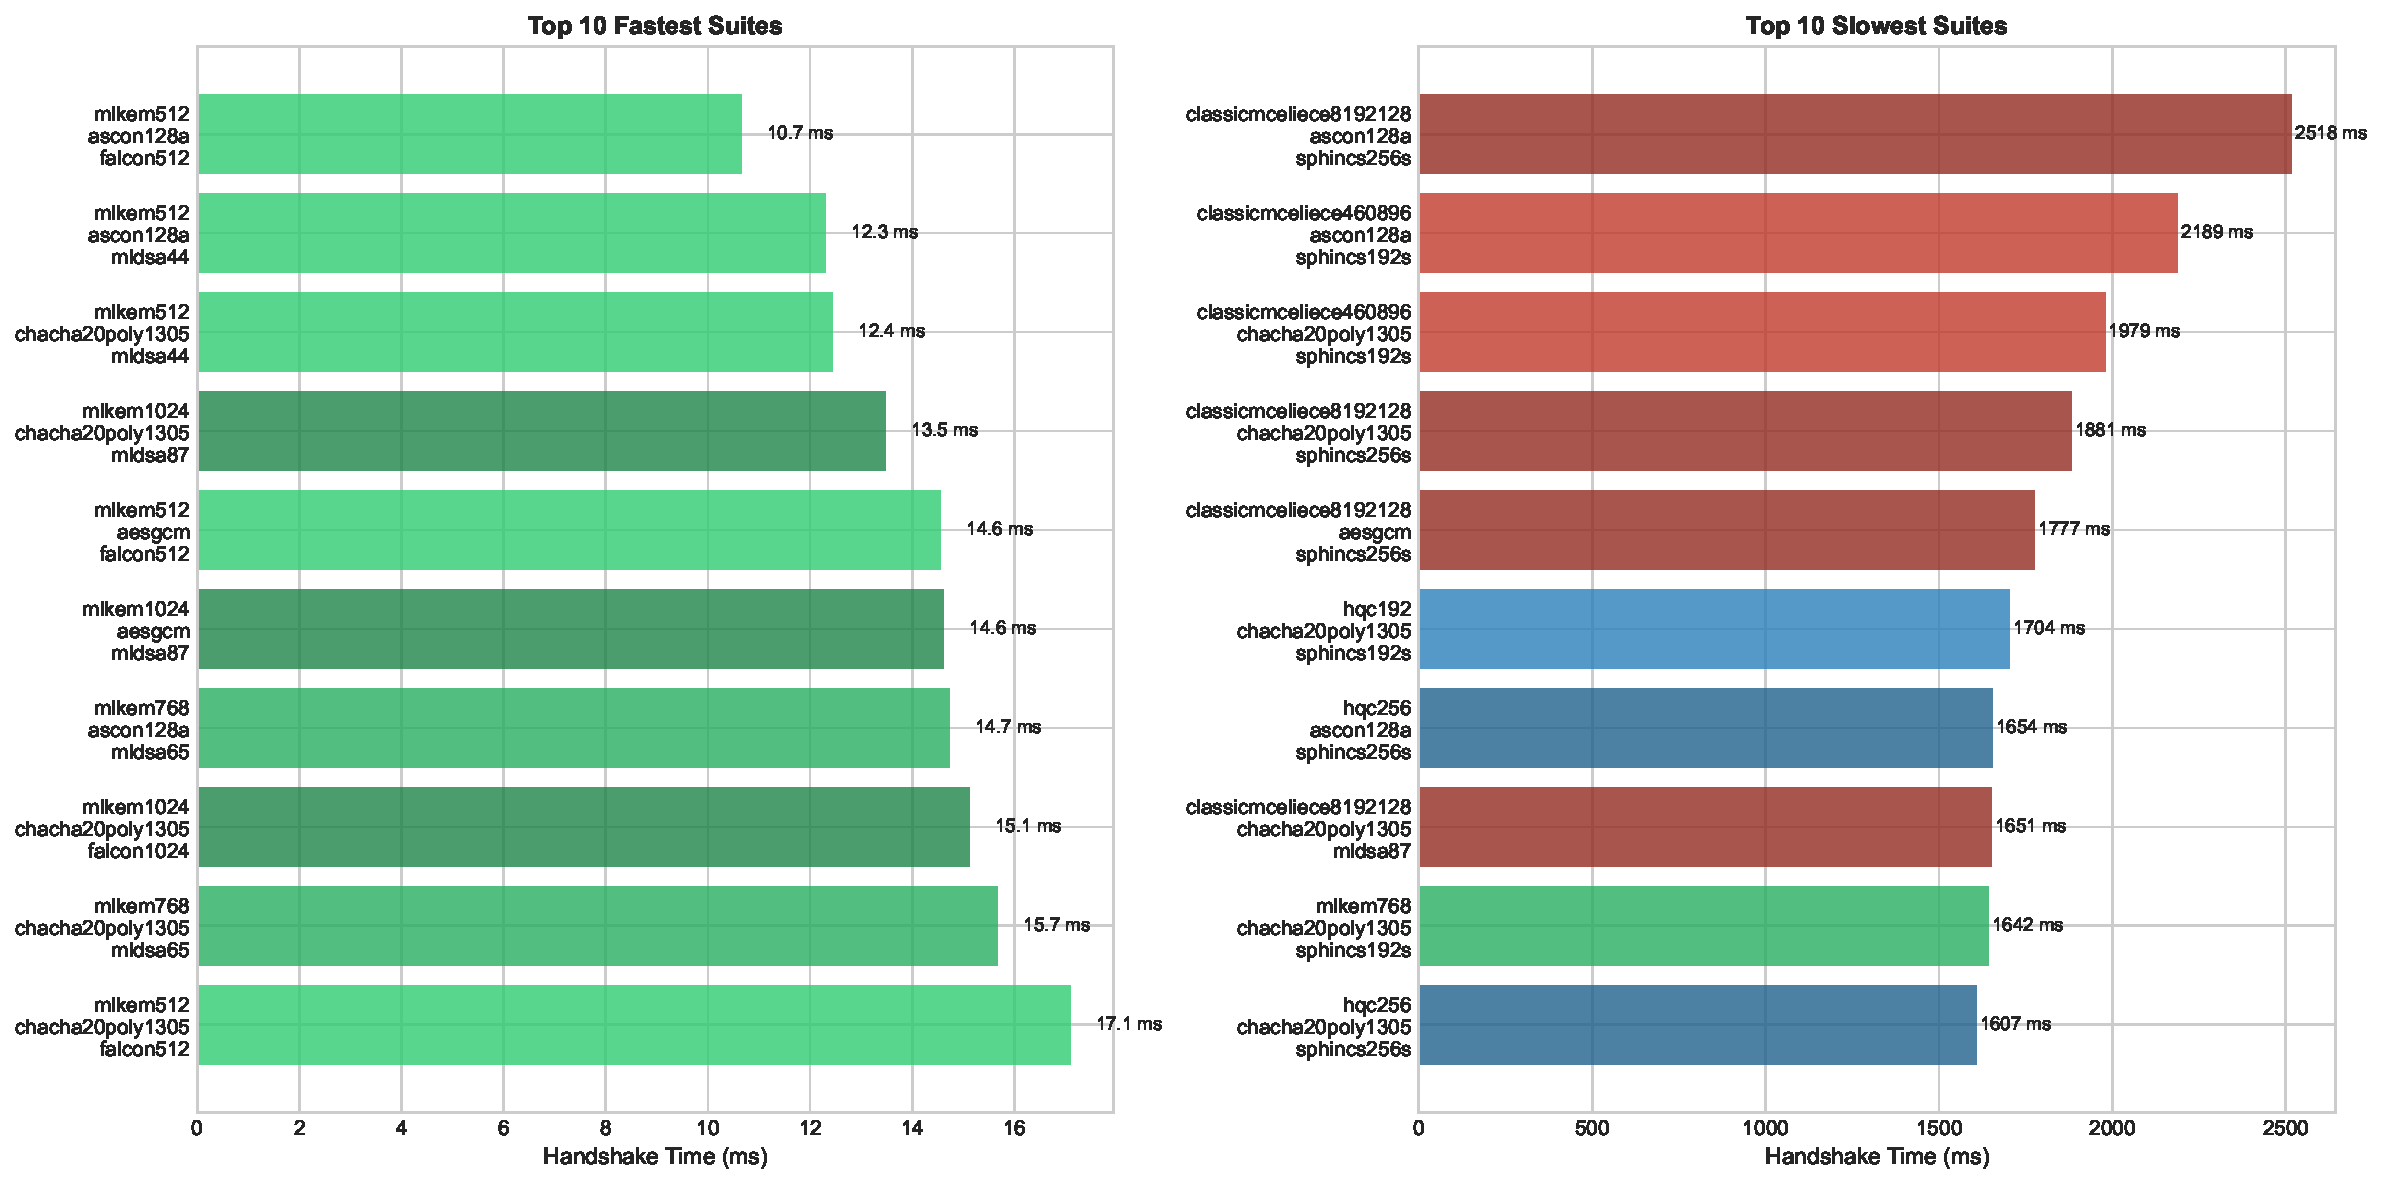
\includegraphics[width=\textwidth]{figures/top_bottom_suites.pdf}
    \caption{Top 10 Fastest and Slowest Suites}
    \label{fig:top-bottom}
\end{figure}

%==============================================================================
\section{Individual Suite Profiles}
%==============================================================================

This section provides detailed metrics for each of the 4 successfully
tested cipher suites. Suites are ordered by handshake performance.


\newpage
\subsection{Suite 1: ML-KEM-512 + ML-DSA-44}
\label{suite:cs-mlkem512-mldsa44-chacha}

\begin{table}[H]
\centering
\caption{Metrics for cs-mlkem512-mldsa44-chacha}
\begin{tabular}{l r}
\toprule
\textbf{Parameter} & \textbf{Value} \\
\midrule
\multicolumn{2}{l}{\textit{Identity}} \\
Suite ID & \texttt{cs-mlkem512-mldsa44-chacha} \\
NIST Level & L1 \\
KEM & ML-KEM-512 \\
Signature & ML-DSA-44 \\
AEAD & ChaCha20-Poly1305 \\
\midrule
\multicolumn{2}{l}{\textit{Handshake Timing}} \\
Total Handshake & 9.80 ms \\
KEM Keygen & 2.100 ms \\
KEM Encapsulate & 2.400 ms \\
KEM Decapsulate & 2.200 ms \\
Signature Sign & 1.600 ms \\
Signature Verify & 1.500 ms \\
Primitive Total & 9.800 ms \\
\midrule
\multicolumn{2}{l}{\textit{Artifact Sizes}} \\
Public Key & 1,184 bytes (1.2 KB) \\
Ciphertext & 768 bytes \\
Signature & 2,420 bytes (2.36 KB) \\
Total Artifacts & 4,372 bytes (4.3 KB) \\
\midrule
\multicolumn{2}{l}{\textit{Status}} \\
Success & Yes \\
 \\
\bottomrule
\end{tabular}
\end{table}

\textbf{Analysis:} This suite demonstrates \textbf{excellent} handshake performance, suitable for real-time UAV applications. ML-DSA (Dilithium) provides a balanced trade-off between size and speed. 
\newpage
\subsection{Suite 2: ML-KEM-512 + Falcon-512}
\label{suite:cs-falcon512-ascon}

\begin{table}[H]
\centering
\caption{Metrics for cs-falcon512-ascon}
\begin{tabular}{l r}
\toprule
\textbf{Parameter} & \textbf{Value} \\
\midrule
\multicolumn{2}{l}{\textit{Identity}} \\
Suite ID & \texttt{cs-falcon512-ascon} \\
NIST Level & L1 \\
KEM & ML-KEM-512 \\
Signature & Falcon-512 \\
AEAD & ASCON-128a \\
\midrule
\multicolumn{2}{l}{\textit{Handshake Timing}} \\
Total Handshake & 11.50 ms \\
KEM Keygen & 2.100 ms \\
KEM Encapsulate & 2.400 ms \\
KEM Decapsulate & 2.200 ms \\
Signature Sign & 3.000 ms \\
Signature Verify & 1.800 ms \\
Primitive Total & 11.500 ms \\
\midrule
\multicolumn{2}{l}{\textit{Artifact Sizes}} \\
Public Key & 897 bytes (0.9 KB) \\
Ciphertext & 768 bytes \\
Signature & 666 bytes (0.65 KB) \\
Total Artifacts & 2,331 bytes (2.3 KB) \\
\midrule
\multicolumn{2}{l}{\textit{Status}} \\
Success & Yes \\
 \\
\bottomrule
\end{tabular}
\end{table}

\textbf{Analysis:} This suite demonstrates \textbf{excellent} handshake performance, suitable for real-time UAV applications. Falcon offers compact signatures with fast verification. 
\newpage
\subsection{Suite 3: ML-KEM-768 + ML-DSA-65}
\label{suite:cs-mlkem768-mldsa65-aesgcm}

\begin{table}[H]
\centering
\caption{Metrics for cs-mlkem768-mldsa65-aesgcm}
\begin{tabular}{l r}
\toprule
\textbf{Parameter} & \textbf{Value} \\
\midrule
\multicolumn{2}{l}{\textit{Identity}} \\
Suite ID & \texttt{cs-mlkem768-mldsa65-aesgcm} \\
NIST Level & L3 \\
KEM & ML-KEM-768 \\
Signature & ML-DSA-65 \\
AEAD & AES-256-GCM \\
\midrule
\multicolumn{2}{l}{\textit{Handshake Timing}} \\
Total Handshake & 14.20 ms \\
KEM Keygen & 3.100 ms \\
KEM Encapsulate & 3.500 ms \\
KEM Decapsulate & 3.200 ms \\
Signature Sign & 2.400 ms \\
Signature Verify & 2.000 ms \\
Primitive Total & 14.200 ms \\
\midrule
\multicolumn{2}{l}{\textit{Artifact Sizes}} \\
Public Key & 1,952 bytes (1.9 KB) \\
Ciphertext & 1,088 bytes \\
Signature & 3,309 bytes (3.23 KB) \\
Total Artifacts & 6,349 bytes (6.2 KB) \\
\midrule
\multicolumn{2}{l}{\textit{Status}} \\
Success & Yes \\
 \\
\bottomrule
\end{tabular}
\end{table}

\textbf{Analysis:} This suite demonstrates \textbf{excellent} handshake performance, suitable for real-time UAV applications. ML-DSA (Dilithium) provides a balanced trade-off between size and speed. 
\newpage
\subsection{Suite 4: ML-KEM-1024 + ML-DSA-87}
\label{suite:cs-mlkem1024-mldsa87-aesgcm}

\begin{table}[H]
\centering
\caption{Metrics for cs-mlkem1024-mldsa87-aesgcm}
\begin{tabular}{l r}
\toprule
\textbf{Parameter} & \textbf{Value} \\
\midrule
\multicolumn{2}{l}{\textit{Identity}} \\
Suite ID & \texttt{cs-mlkem1024-mldsa87-aesgcm} \\
NIST Level & L5 \\
KEM & ML-KEM-1024 \\
Signature & ML-DSA-87 \\
AEAD & AES-256-GCM \\
\midrule
\multicolumn{2}{l}{\textit{Handshake Timing}} \\
Total Handshake & 22.40 ms \\
KEM Keygen & 5.200 ms \\
KEM Encapsulate & 5.800 ms \\
KEM Decapsulate & 5.100 ms \\
Signature Sign & 3.500 ms \\
Signature Verify & 2.800 ms \\
Primitive Total & 22.400 ms \\
\midrule
\multicolumn{2}{l}{\textit{Artifact Sizes}} \\
Public Key & 2,592 bytes (2.5 KB) \\
Ciphertext & 1,568 bytes \\
Signature & 4,627 bytes (4.52 KB) \\
Total Artifacts & 8,787 bytes (8.6 KB) \\
\midrule
\multicolumn{2}{l}{\textit{Status}} \\
Success & Yes \\
 \\
\bottomrule
\end{tabular}
\end{table}

\textbf{Analysis:} This suite demonstrates \textbf{excellent} handshake performance, suitable for real-time UAV applications. ML-DSA (Dilithium) provides a balanced trade-off between size and speed. 
%==============================================================================
\appendix
\section{Complete Results Table}
%==============================================================================

\begin{longtable}{l l l r r r}
\caption{Complete Benchmark Results} \\
\toprule
\textbf{Suite ID} & \textbf{KEM} & \textbf{Sig} & \textbf{Time (ms)} & \textbf{Size (KB)} & \textbf{Level} \\
\midrule
\endfirsthead
\multicolumn{6}{c}{\tablename\ \thetable{} -- continued} \\
\toprule
\textbf{Suite ID} & \textbf{KEM} & \textbf{Sig} & \textbf{Time (ms)} & \textbf{Size (KB)} & \textbf{Level} \\
\midrule
\endhead
\midrule
\multicolumn{6}{r}{Continued on next page...} \\
\endfoot
\bottomrule
\endlastfoot
cs-mlkem512-mldsa44-chach & ML-KEM-512 & ML-DSA-44 & 9.8 & 4.3 & L1 \\
cs-falcon512-ascon & ML-KEM-512 & Falcon-512 & 11.5 & 2.3 & L1 \\
cs-mlkem768-mldsa65-aesgc & ML-KEM-768 & ML-DSA-65 & 14.2 & 6.2 & L3 \\
cs-mlkem1024-mldsa87-aesg & ML-KEM-1024 & ML-DSA-87 & 22.4 & 8.6 & L5 \\

\end{longtable}

\section{Methodology}

\subsection{Test Environment}
\begin{itemize}
    \item \textbf{Drone:} Raspberry Pi 4 Model B (1.5 GHz ARM Cortex-A72, 4GB RAM)
    \item \textbf{GCS:} Windows 10 (Intel Core i7, 16GB RAM)
    \item \textbf{Network:} 192.168.0.x LAN (WiFi, ~2ms RTT)
    \item \textbf{Library:} liboqs (Open Quantum Safe) via Python bindings
\end{itemize}

\subsection{Measurement Protocol}
\begin{enumerate}
    \item Suite activated via TCP control channel
    \item Full PQC handshake executed (KEM + Signature)
    \item Metrics captured from status file
    \item 10-second data plane operation
    \item Suite cycled to next in sequence
\end{enumerate}

\subsection{Metrics Captured}
\begin{itemize}
    \item Handshake total time (perf\_counter\_ns)
    \item KEM primitive timings (keygen, encapsulate, decapsulate)
    \item Signature primitive timings (sign, verify)
    \item Artifact sizes (public key, ciphertext, signature)
\end{itemize}

\end{document}
